\documentclass[12pt,]{article}
\usepackage{lmodern}
\usepackage{amssymb,amsmath}
\usepackage{ifxetex,ifluatex}
\usepackage{fixltx2e} % provides \textsubscript
\ifnum 0\ifxetex 1\fi\ifluatex 1\fi=0 % if pdftex
  \usepackage[T1]{fontenc}
  \usepackage[utf8]{inputenc}
\else % if luatex or xelatex
  \ifxetex
    \usepackage{mathspec}
  \else
    \usepackage{fontspec}
  \fi
  \defaultfontfeatures{Ligatures=TeX,Scale=MatchLowercase}
    \setmainfont[]{Times New Roman}
\fi
% use upquote if available, for straight quotes in verbatim environments
\IfFileExists{upquote.sty}{\usepackage{upquote}}{}
% use microtype if available
\IfFileExists{microtype.sty}{%
\usepackage{microtype}
\UseMicrotypeSet[protrusion]{basicmath} % disable protrusion for tt fonts
}{}
\usepackage[margin=2.54cm]{geometry}
\usepackage{hyperref}
\hypersetup{unicode=true,
            pdftitle={Trend Analysis and Predictors of Lake Level Changes in Lake Tahoe, CA},
            pdfauthor={Nikki Shintaku},
            pdfborder={0 0 0},
            breaklinks=true}
\urlstyle{same}  % don't use monospace font for urls
\usepackage{longtable,booktabs}
\usepackage{graphicx,grffile}
\makeatletter
\def\maxwidth{\ifdim\Gin@nat@width>\linewidth\linewidth\else\Gin@nat@width\fi}
\def\maxheight{\ifdim\Gin@nat@height>\textheight\textheight\else\Gin@nat@height\fi}
\makeatother
% Scale images if necessary, so that they will not overflow the page
% margins by default, and it is still possible to overwrite the defaults
% using explicit options in \includegraphics[width, height, ...]{}
\setkeys{Gin}{width=\maxwidth,height=\maxheight,keepaspectratio}
\IfFileExists{parskip.sty}{%
\usepackage{parskip}
}{% else
\setlength{\parindent}{0pt}
\setlength{\parskip}{6pt plus 2pt minus 1pt}
}
\setlength{\emergencystretch}{3em}  % prevent overfull lines
\providecommand{\tightlist}{%
  \setlength{\itemsep}{0pt}\setlength{\parskip}{0pt}}
\setcounter{secnumdepth}{5}
% Redefines (sub)paragraphs to behave more like sections
\ifx\paragraph\undefined\else
\let\oldparagraph\paragraph
\renewcommand{\paragraph}[1]{\oldparagraph{#1}\mbox{}}
\fi
\ifx\subparagraph\undefined\else
\let\oldsubparagraph\subparagraph
\renewcommand{\subparagraph}[1]{\oldsubparagraph{#1}\mbox{}}
\fi

%%% Use protect on footnotes to avoid problems with footnotes in titles
\let\rmarkdownfootnote\footnote%
\def\footnote{\protect\rmarkdownfootnote}

%%% Change title format to be more compact
\usepackage{titling}

% Create subtitle command for use in maketitle
\providecommand{\subtitle}[1]{
  \posttitle{
    \begin{center}\large#1\end{center}
    }
}

\setlength{\droptitle}{-2em}

  \title{Trend Analysis and Predictors of Lake Level Changes in Lake Tahoe, CA}
    \pretitle{\vspace{\droptitle}\centering\huge}
  \posttitle{\par}
  \subtitle{\url{https://github.com/nmshintaku/Data_Analytics_final_project}}
  \author{Nikki Shintaku}
    \preauthor{\centering\large\emph}
  \postauthor{\par}
    \date{}
    \predate{}\postdate{}
  
\usepackage{float}
\let\origfigure\figure
\let\endorigfigure\endfigure
\renewenvironment{figure}[1][2] {
    \expandafter\origfigure\expandafter[H]
} {
    \endorigfigure
}

\begin{document}
\maketitle

\begin{figure}
\centering
\includegraphics{Tahoe.png}
\caption{Lake Tahoe, CA}
\end{figure}

\newpage
\tableofcontents 
\newpage
\listoftables 
\newpage
\listoffigures 
\newpage

\hypertarget{rationale-and-research-questions}{%
\section{Rationale and Research
Questions}\label{rationale-and-research-questions}}

Lake Tahoe measures at 6,220 feet above sea level, and is 22 miles long
and 12 miles wide spanning across the California-Nevada state border.
Lake Tahoe water is 99.994\% pure contributing to its legendary and
beautiful water clarity. However, Lake Tahoe is facing decline of water
clarity and health from the impacts of climate change, invasive species,
and pollution. Climate change is causing more precipitation to fall as
rain rather than snow, which leads to increase stormwater runoff
carrying sediment into Lake Tahoe. In addition, California is
experiencing extended droughts affecting amount of annual precipitation.
Inadvertently, climate change is also increasing the lake's water
temperature and affecting regional weather patterns that could change
the lake's ecosystem. Snowmelt from 63 tributaries in the watershed adds
65\% of Lake Tahoe's water, and the other 35\% falls as precipitation
directly in the lake.

Lake Tahoe's water level is controlled at the Tahoe City Dam, its only
outlet. The legal limit for water above the natural rim at that dam is
6,229.1 ft. If the lake reaches its legal limit, flooding would begin to
impact the area along with damage from erosion. With the unforeseeable
consequences of climate change and the task to keep water levels below
maximum legal limit, it is important to understand what atmospheric
factors play a role in Lake Tahoe's water level.

This analysis investigates the trends in Lake Tahoe's water level and
the possible drivers of lake level accross the time period of 1957 -
2019 through the research questions:

\begin{enumerate}
\def\labelenumi{\arabic{enumi}.}
\item
  How does lake level in Lake Tahoe change over the years? Is there an
  increasing or decreasing trend in lake level over time?
\item
  What are significant atmospheric predictors of lake level in Lake
  Tahoe?
\end{enumerate}

The gage station site for measuring lake water level (or gage height) is
located in Tahoe City, CA where the dam is controlled, and the data was
downloaded from USGS. Subsequent atmospheric data includes
precipitation, snow fall, snow depth, average daily temperature, maximum
daily temperature, and minimum daily temperature downloaded from NOAA
and subsetted to the Tahoe City, CA station to be as accurate as
possible for data collection location.

\emph{Fun Fact: If you were to pour Lake Tahoe out onto an area the size
of California, the water would still be 14 inches deep.}

\newpage

\hypertarget{dataset-information}{%
\section{Dataset Information}\label{dataset-information}}

\hypertarget{usgs-gage-height-data}{%
\subsection{USGS Gage Height Data}\label{usgs-gage-height-data}}

The data for lake level was downloaded from USGS Water-Quality Data for
the Nation website at \url{https://waterdata.usgs.gov/nwis/qw}. The
dataset contains daily gage height measurements in feet from January
1920 - December 2019 from one station (Site \#103370000) in Tahoe City,
CA. USGS reports that gage height is measured from the recorded lake
elevation of 6,220 ft as the zero baseline. Gage height measurement +
current lake elevation (6,220 ft) will give the actual lake level from
sea level.

This dataset was relatively easy to wrangle; unneccesary columns were
dropped, leaving only date and gage height. There was a time period from
January 1920 - April 1920 with gage height measurements, and then no
measurements until October 1, 1957 so a decision was made to remove the
3 months of data in 1920 because the gap between 1920 and 1957 is too
large to interpolate daily measurements. Furthermore, the three months
of data is too short of a time period to do a time series analysis.
After that wranging, there were 3 gage height NAs so these were linearly
interpolated to create a complete dataset.

\begin{longtable}[]{@{}ll@{}}
\caption{\label{tab:table} USGS Gage Height Data Summary}\tabularnewline
\toprule
Data & Summary\tabularnewline
\midrule
\endfirsthead
\toprule
Data & Summary\tabularnewline
\midrule
\endhead
Total Number of Samples & 22,737\tabularnewline
Start Date & 1957-10-01\tabularnewline
End Date & 2019-12-31\tabularnewline
Gage Height Mean (ft) & 5.86\tabularnewline
Gage Height Median (ft) & 6.32\tabularnewline
Gage Height Min (ft) & 0.26\tabularnewline
Gage Height Max (ft) & 9.40\tabularnewline
\bottomrule
\end{longtable}

\hypertarget{noaa-climate-data}{%
\subsection{NOAA Climate Data}\label{noaa-climate-data}}

The atmospheric data was downloaded from NOAA National Centers for
Environmental Information at \url{https://www.ncdc.noaa.gov/cdo-web/}.
This dataset contains daily measurements for precipitation, snow fall,
snow depth, average daily temperature, maximum daily temperature, and
minimum daily temperature beginning from September 13, 1903 - March 30,
2020 from 5 different stations within the zip code of 96145 (for Tahoe
City, CA). Precipitation, snowfall, and snow depth are measured in
inches, and temperatures are all measured in fahrenheit.

With such a large time period for this dataset, there is a lot of NAs
and an uneven amount of measurements across the stations. To be as
accurate as possible for location of both the gage height station and
climate station, the station named ``TAHOE CITY, CA US'' was filterd out
to be used in this analysis. The data for the Tahoe City station ranges
from September 13, 1903 - March 30, 2020 so the dates were filtered to
match the same time period as the gage height measurements from October
1, 1957 - December 31, 2019. From here, presence of NAs were checked,
and the entire column for average daily temperature was NAs so that
column was deleted entirely. The rest of the data with NAs were linearly
interpolated to create a complete dataset.

\begin{longtable}[]{@{}llllll@{}}
\caption{\label{tab:table} NOAA Tahoe City Climate Data
Summary}\tabularnewline
\toprule
Variable & Date & Mean & Median & Min & Max\tabularnewline
\midrule
\endfirsthead
\toprule
Variable & Date & Mean & Median & Min & Max\tabularnewline
\midrule
\endhead
Start Date & 1957-10-01 & - & - & - & -\tabularnewline
End Date & 2019-12-31 & - & - & - & -\tabularnewline
Precipitation (in) & - & 0.09 & 0 & 0 & 6.77\tabularnewline
Snow Fall (in) & - & 0.49 & 0 & 0 & 42\tabularnewline
Snow Depth (in) & - & 7.74 & 0 & 0 & 120\tabularnewline
Daily Temp Max (F) & - & 56.82 & 55 & 11 & 94\tabularnewline
Daily Temp Min (F) & - & 31.35 & 31 & -16 & 79\tabularnewline
\bottomrule
\end{longtable}

Lastly, the USGS processed data and the NOAA Tahoe City climate
processed data were joined together by date to create a large dataset
containing gage height and climate data together. For data explorataion
and visualization purposes, temperature in celsisus was calculated for
minimum and maximum daily temperatures.

\newpage

\hypertarget{exploratory-analysis}{%
\section{Exploratory Analysis}\label{exploratory-analysis}}

To visualize what all the data looks like across time, each variable was
plotted side by side using the original dates provided. Figure 2 shows
the six variables that the analysis is investigating. It is clear in
Graph A that gage height measurements are available beginning in the
late 1950s to present. The gage height data indicates an oscillation
pattern from high lake level to low lake level throughout the years. The
NOAA climate data is graphed starting from the early 1900s, and there
are some clear data gaps in precipitation (Graph B) and snow depth
(Graph D). Graph E and F represent the daily temperatures in degrees
celsisus with the red color symbolizing positive temperatures and the
blue color symbolizing negative temperatures. Out of the NOAA climate
data, there is no comprehensible pattern throughout the time period.

\begin{figure}
\centering
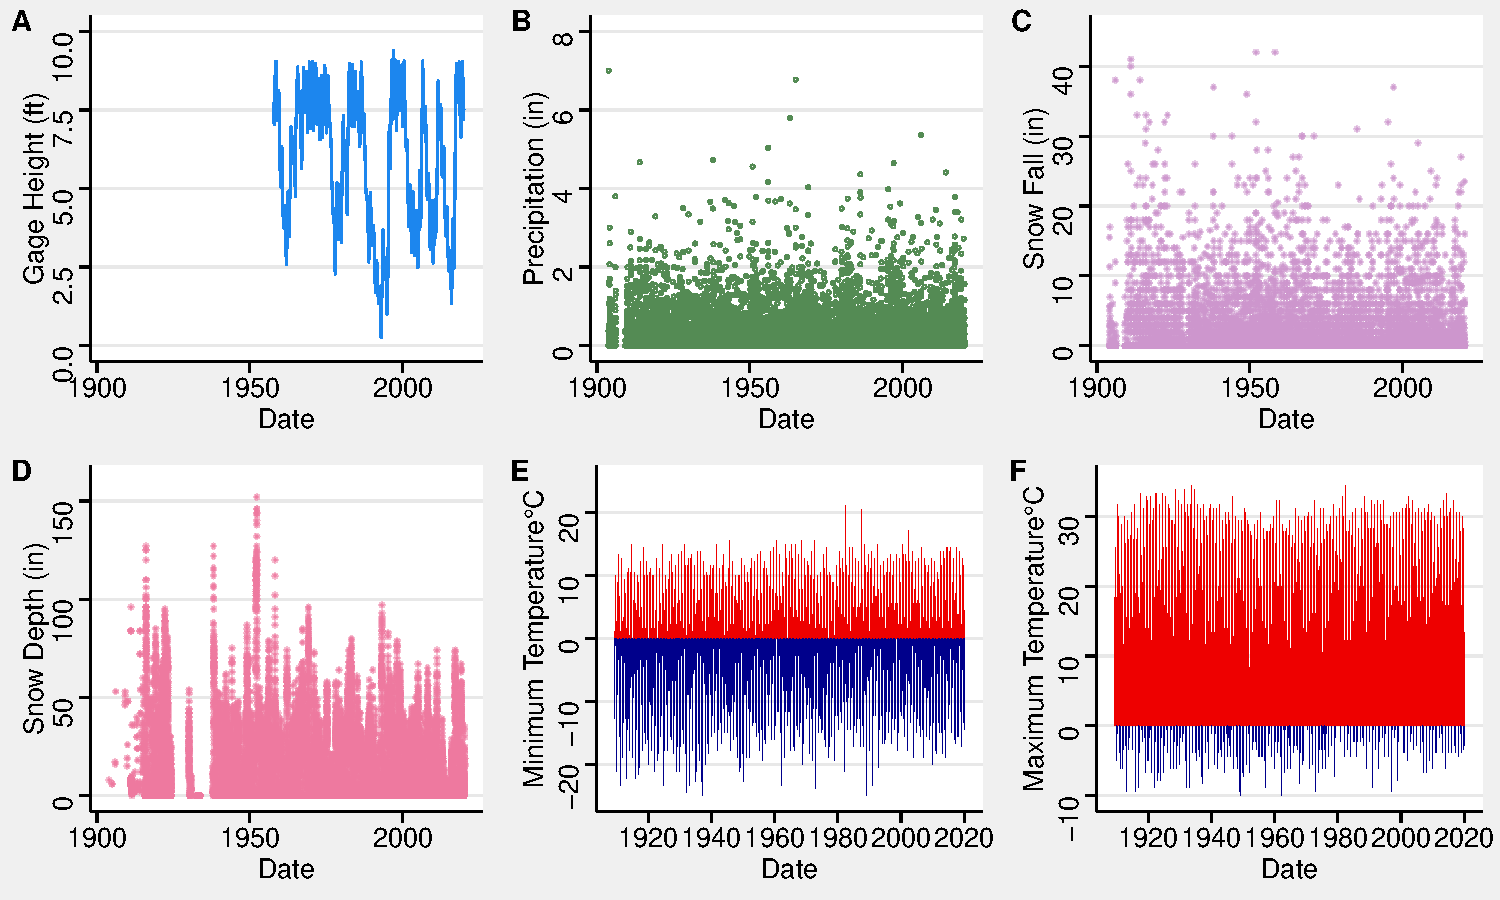
\includegraphics{Shintaku_ENV872_Project_files/figure-latex/unnamed-chunk-3-1.pdf}
\caption{Lake Tahoe Gage Height and Climate Data Time Series 1903-2019}
\end{figure}

Because this analysis is looking at predictors of gage height (or lake
level), the NOAA climate data was cut to match the same dates as the
USGS data for 1957 - 2019. Figure 3 shows the distribution of the six
variables across those years. Again, out of the NOAA climate data, there
is no comprehensible pattern throughout the time period.

\begin{figure}
\centering
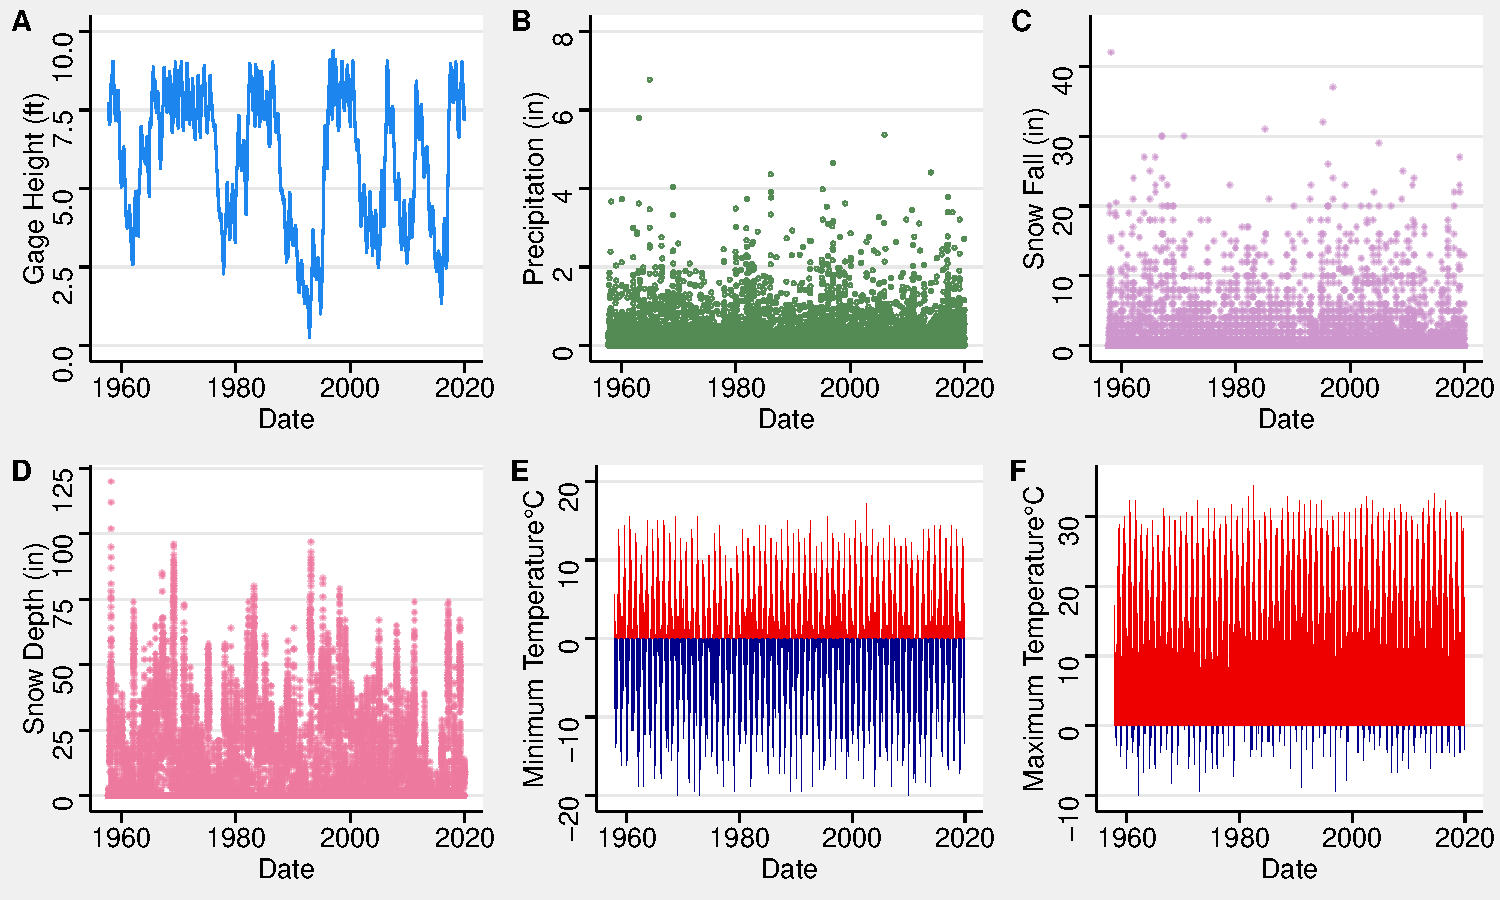
\includegraphics{Shintaku_ENV872_Project_files/figure-latex/unnamed-chunk-5-1.pdf}
\caption{Lake Tahoe Gage Height and Climate Data Time Series 1957-2019}
\end{figure}

\begin{figure}
\centering
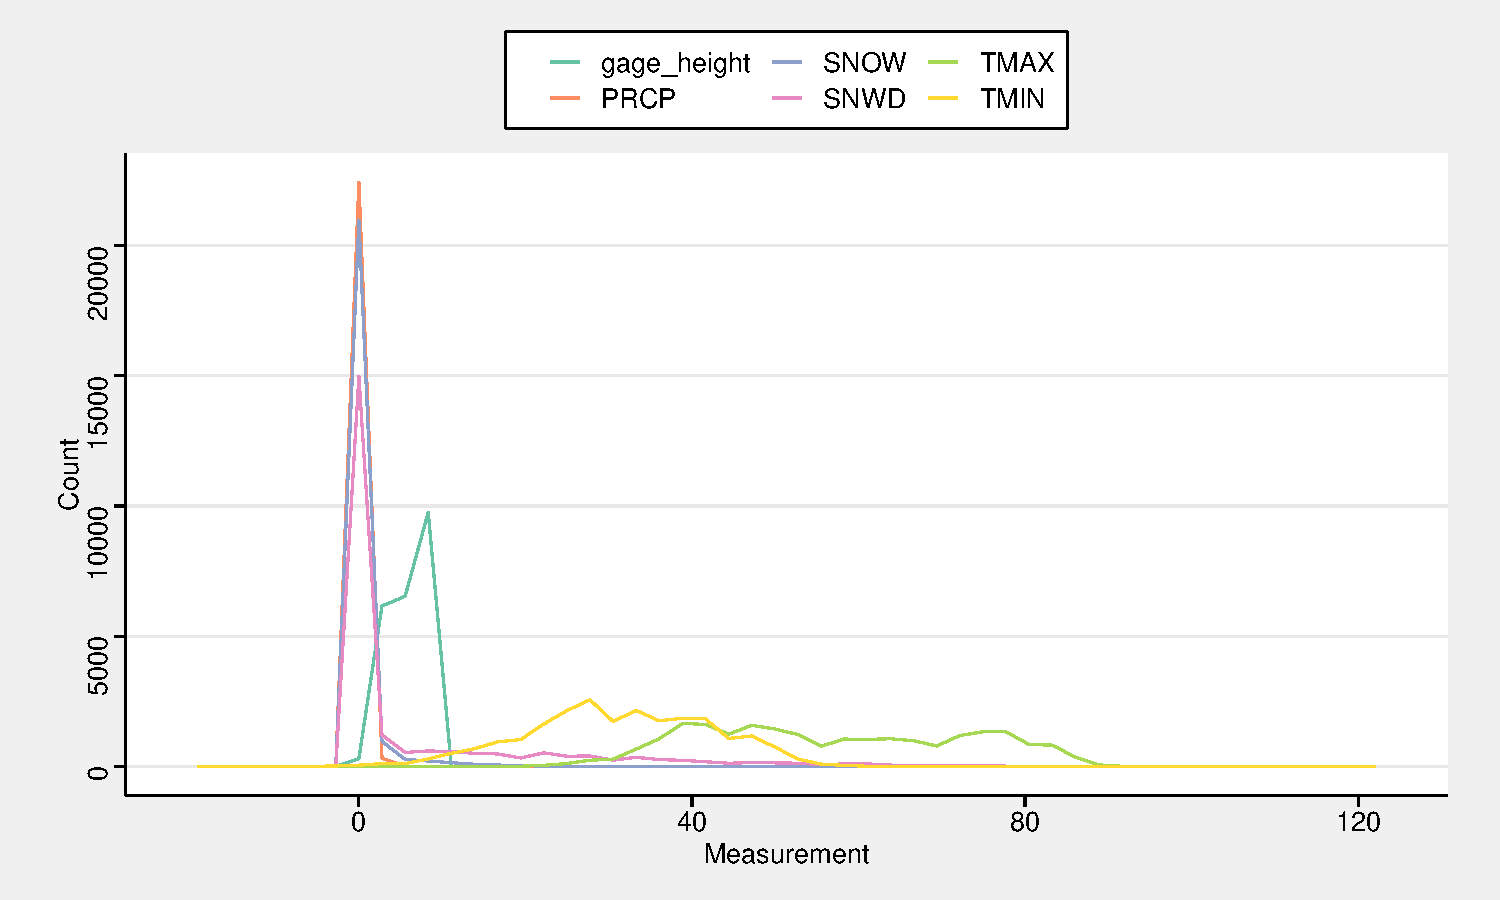
\includegraphics{Shintaku_ENV872_Project_files/figure-latex/unnamed-chunk-6-1.pdf}
\caption{Frequency Polygons Plot of Gage Height and Climate Data}
\end{figure}

A frequency polygon graph was created to view how many observations
occurred for each measurement divided among 50 bins on the x-axis.
Figure 4 shows that precipitation, snow, and snow depth had the highest
observations with measurements closest to 0. Minimum temperatures ranged
from 30-40 degrees F being the most observations, and maximum
temperatures ranged from 40-80 degrees F. Gage height topped count
around a measurement of 7-10. This frequency polygons graph is useful to
compare each of our variables to each other and gives a good overview of
where the majority of the measurements lies.

\newpage

\hypertarget{analysis}{%
\section{Analysis}\label{analysis}}

This study investigates trends of water level of Lake Tahoe using a
\emph{Time Series} analysis and explores significant atmospheric factors
of changing water level using a \emph{Generalized Linear Models}
approach.

\hypertarget{question-1-how-does-lake-level-in-lake-tahoe-change-over-the-years}{%
\subsection{Question 1: How does lake level in Lake Tahoe change over
the
years?}\label{question-1-how-does-lake-level-in-lake-tahoe-change-over-the-years}}

Time series is when a response variable is tracked over time. This time
series will include an explanatory time component and a response
variable (gage height). Time series come with some challenges that need
to be addressed when performing the analysis. Time series do not deal
with data gaps well; missing data in this dataset has already been taken
care of through linear interpolation. In addition, seasonality, which
are cyclic patterns in variables that occur at regular intervals, could
affect interpretation of a monotonic trend. This analysis will take
seasonality into consideration for gage height data.

Times series are made up of several components:

\begin{itemize}
\tightlist
\item
  Seasonal Component: repetition over a fixed known period
\item
  Trend Component: quantifies upward or downward progression over time;
  does not have to be monotonic
\item
  Error/Random Component: the remainder of the time series after the
  other components are accounted for; reflects noise in the dataset
\end{itemize}

Lake water level (gage height) is measured daily at the Tahoe City gage
station. Since the data is one location measured over time, this is a
great dataset for time series analysis.

\begin{figure}
\centering
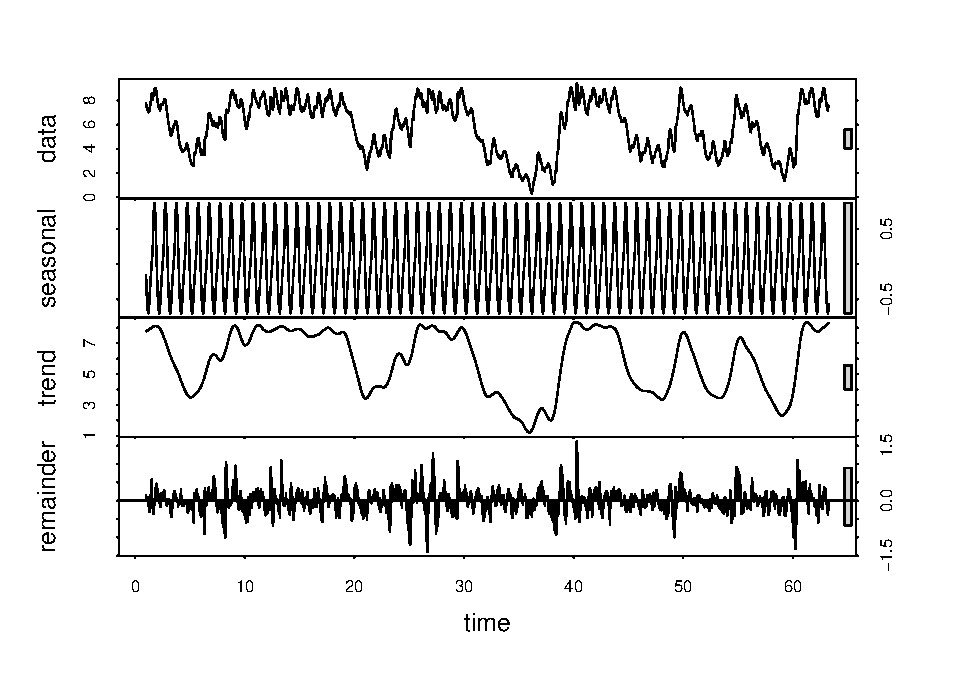
\includegraphics{Shintaku_ENV872_Project_files/figure-latex/unnamed-chunk-7-1.pdf}
\caption{Lake Tahoe Gage Height Time Series Decomposed}
\end{figure}

Figure 5 shows the decomposed components of the time series for gage
height. The grey boxes on the right show the relative size of the y axis
data to each other. The data component is the result of the seasonal
component plus the trend component, and the remainder is left over data
that doesn't fit in either seasonal or trend. Seasonal component is
extracted from 365 days and represents a repeated cycle.

\begin{figure}
\centering
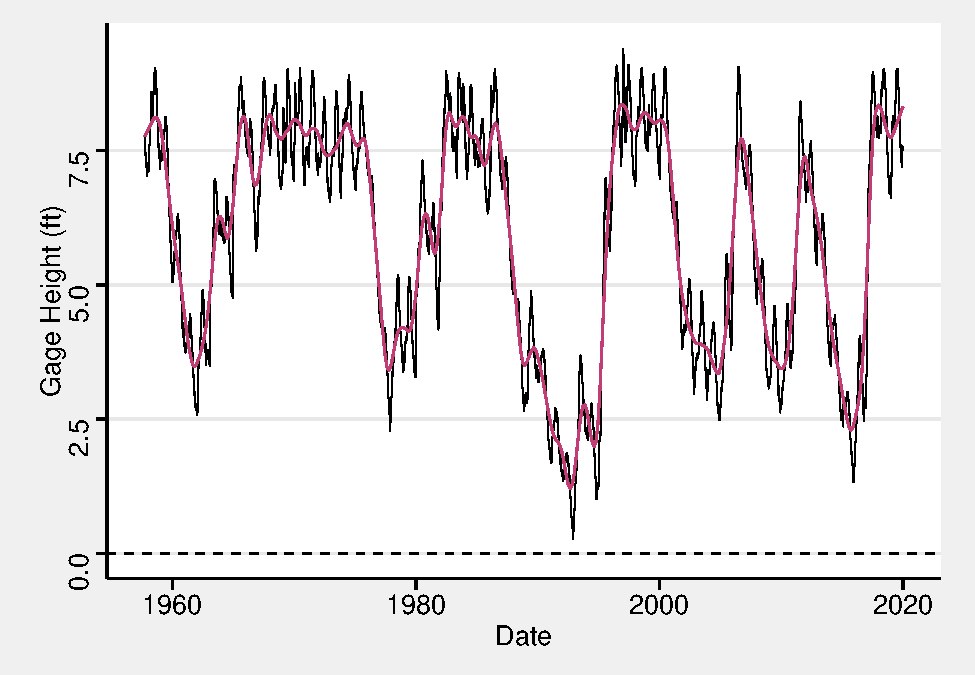
\includegraphics{Shintaku_ENV872_Project_files/figure-latex/unnamed-chunk-8-1.pdf}
\caption{Trend Component Against Actual Data}
\end{figure}

\begin{figure}
\centering
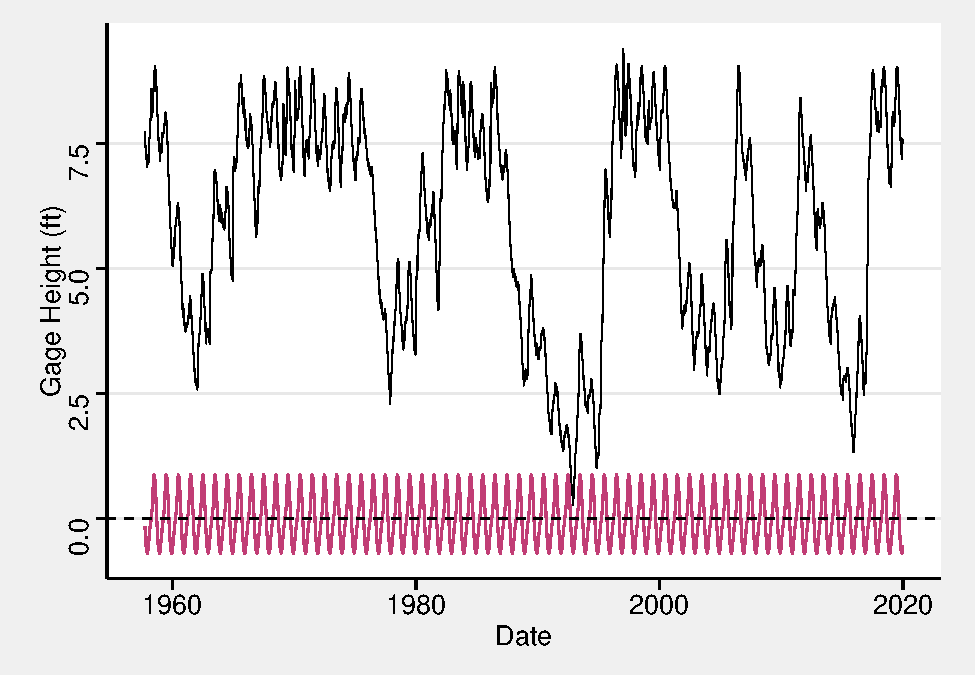
\includegraphics{Shintaku_ENV872_Project_files/figure-latex/unnamed-chunk-9-1.pdf}
\caption{Seasonal Component Against Actual Data}
\end{figure}

Figures 6 and 7 shows the trend and seasonal decomposed components
against the original gage height data. The decomposition is not
constrained by a lower bound of zero, which is why Figure 7 shows the
seasonal component going below zero. In this case, the gage height could
go below zero because its baseline is lake elevation at 6,220 ft. If
gage height were to go below zero, it would likely imply a drought.

For trend analysis, this study considers a monotonic trend. Monotonic
trends are a gradual shift over time that is consistent in direction,
for example in response to climate change. The monotonic analysis in
this study uses a Seasonal Mann-Kendall test. \textbf{Seasonal
Mann-Kendall} assumes seasonality, non-parametric, no temporal
autocorelation, and identical distribution.

We are interested in knowing how lake level has changed over time while
incorporating the seasonal component. The Seasonal Mann-Kendall assumes
no temporal autocorrelation, but daily data is prone to temporal
autocorrelation. In this case,the data is collasped down into monthly
data to (1) reduce temporal autocorrelation and (2) break down the
potential seasonal trend into more interpretable components. Monthly
mean gage height was calculated for this test.

The Seasonal Mann-Kendall test resulted in a significant trend with lake
level over time in Lake Tahoe (Seasonal Mann-Kendall, z = -5.9414,
p-value = 2.827e-09). Since there is a significant trend present,
\emph{Sen's Slope} was computed to quantify the trend. Sen's slope
indicates a decreasing trend over time of -0.0021 as shown on Figure 7
(Sen's Slope, z = -5.955, p-value = 2.601e-09).

\begin{figure}
\centering
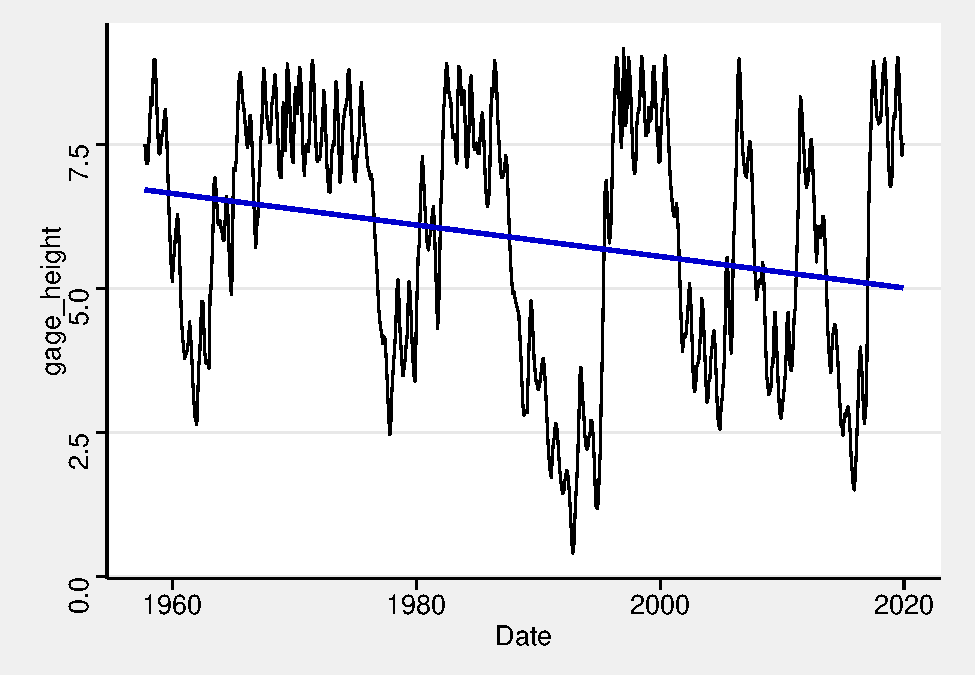
\includegraphics{Shintaku_ENV872_Project_files/figure-latex/unnamed-chunk-11-1.pdf}
\caption{Monthly Mean Gage Height Data with Sen's Slope Trend}
\end{figure}

Pettitt's test was run on the Tahoe gage height monthly time series to
detect change points in lake levels over time as shown in Figure 9. The
first change point occurred most likely around 1987 and the second
change point occurring in 1992. In between Change Point 1 and Change
Point 2, the gage height is the lowest its ever been in displayed time
period; this likely corresponds to the 1987-1992 drought in California
that lasted six years. In addition, there was a five year drought from
2012-2016, which likely corresponds to Change Point 4 when the drought
ends.

\begin{figure}
\centering
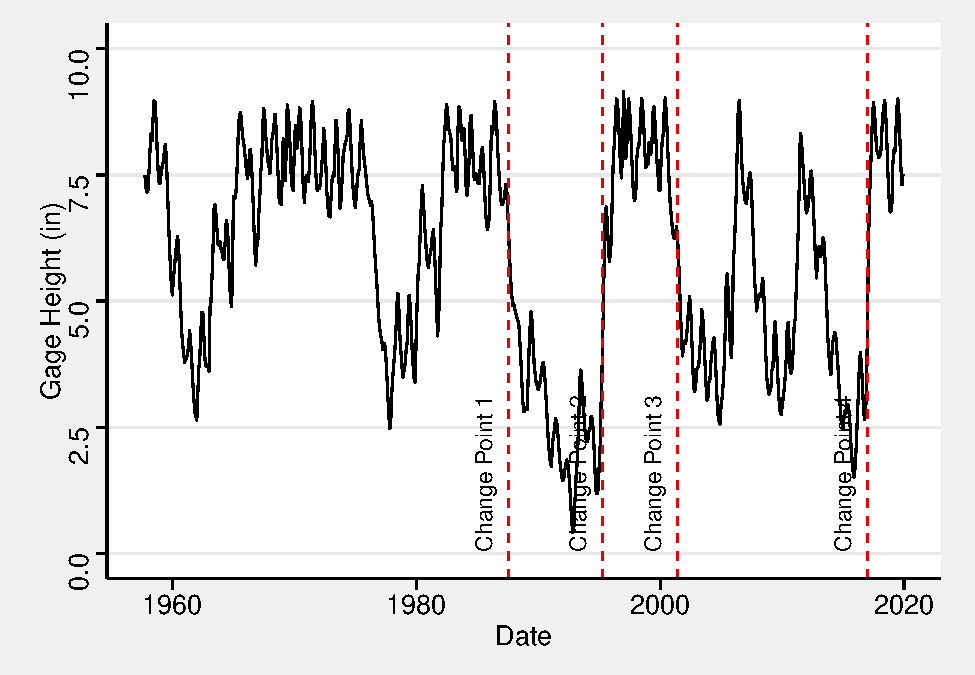
\includegraphics{Shintaku_ENV872_Project_files/figure-latex/unnamed-chunk-12-1.pdf}
\caption{Change points in lake level}
\end{figure}

\hypertarget{question-2-what-are-significant-atmospheric-predictors-of-lake-level-in-lake-tahoe}{%
\subsection{Question 2: What are significant atmospheric predictors of
lake level in Lake
Tahoe?}\label{question-2-what-are-significant-atmospheric-predictors-of-lake-level-in-lake-tahoe}}

In order to find significant atmospheric predictors of lake level,
generalized linear modeling (GLM) was used through linear regression. A
linear regression is formed of a continuous response variable plus a
combination of 1+ continuous response variables (and the error term).
The equation is an algebraic expression:
\[y = \alpha + \beta*x + \epsilon \]

The goal of linear regression is to find the line of best fit that
minimizes the total distance of points from the line. With GLM comes
some assumptions:

\begin{itemize}
\tightlist
\item
  Data resisduals approximate a normal distribution
\item
  Variance in response variable is equal among groups (for analyzing
  categorical explanatory variables)
\end{itemize}

This investigation computes both simple linear regression and multiple
linear regression.

\hypertarget{simple-linear-regression}{%
\subsubsection{Simple Linear
Regression}\label{simple-linear-regression}}

\textbf{Single Linear Regression} is with a continuous response and one
continuous explanatory variable. Simple linear regressions were run on
each of the five climate variables to test if a single variable is a
signficant predictor of lake level. For the purpose of this study, only
the two best models will be presented and analyzed.

\hypertarget{daily-minimum-temperature-as-a-significant-predictor}{%
\paragraph{Daily Minimum Temperature as a Significant
Predictor}\label{daily-minimum-temperature-as-a-significant-predictor}}

Can we predict lake level from minimum temperature? After running the
simple linear regression, minimum temperature is a significant predictor
of lake level (Simple Linear Regression, df = 22732, p-value =
\textless{} 2.2e-16, R2 = 0.025). For every 1 degree F increase in
minimum temperature, there is an increase in gage height by 0.032 ft,
and minimum temperature accounts for 2.5\% of the variance in lake
level. There is a significant positive correlation between minimum
temperautre and lake level (Correlation, df = 22732, p-value = 2.2e-16,
cor = 0.159). Figure 10 shows minimum temperature by gage height with
the linear regression trend line in black.

\[Gage Height = 4.87 + 0.032*Tmin \]

\begin{figure}
\centering
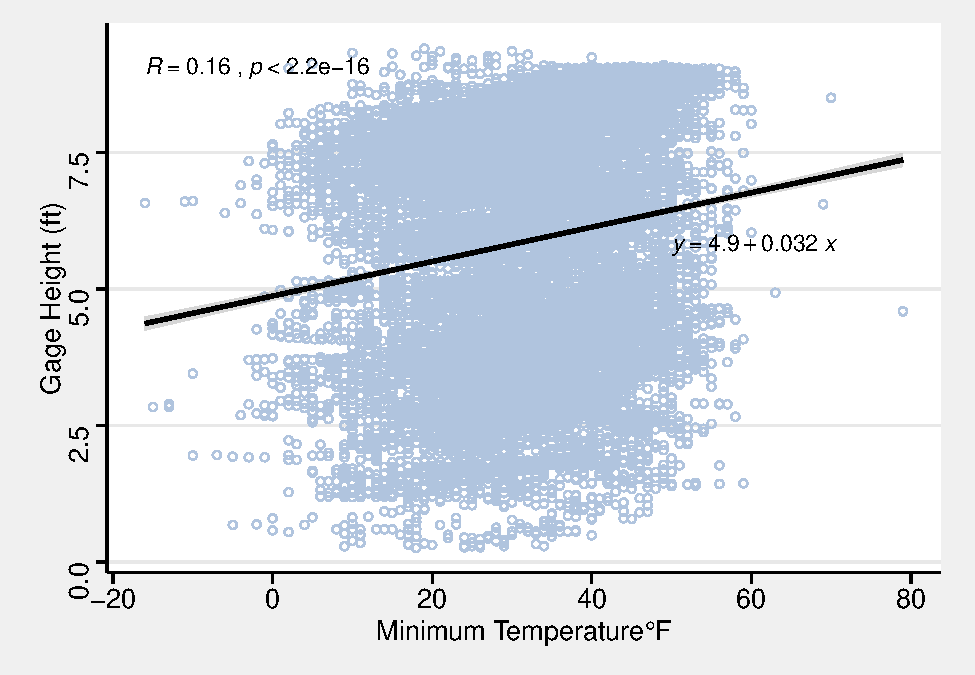
\includegraphics{Shintaku_ENV872_Project_files/figure-latex/unnamed-chunk-13-1.pdf}
\caption{Minimum temperature by gage height with trend line in black}
\end{figure}

\hypertarget{daily-maximum-temperature-as-a-significant-predictor}{%
\paragraph{Daily Maximum Temperature as a Significant
Predictor}\label{daily-maximum-temperature-as-a-significant-predictor}}

Can we predict lake level from maximum temperature? Maximum temperature
is also a significant predictor of lake level (Simple Linear Regression,
df = 22732, p-value = 2.2e-16, R2 = 0.011). For every 1 degree F
increase in maximum temperature, there is an increse in gage height by
0.014 ft, and maximum temperature accounts for 1.1\% of variance in lake
level. There is a significnat positive correlation between maximum
temperautre and lake level (Correlation, df = 22732, p-value = 2.2e-16,
cor = 0.105). Figure 11 shows maximum temperature by gage height with
the linear regression trend line in black.

\[Gage Height = 5.042 + 0.014*Tmax \]

\begin{figure}
\centering
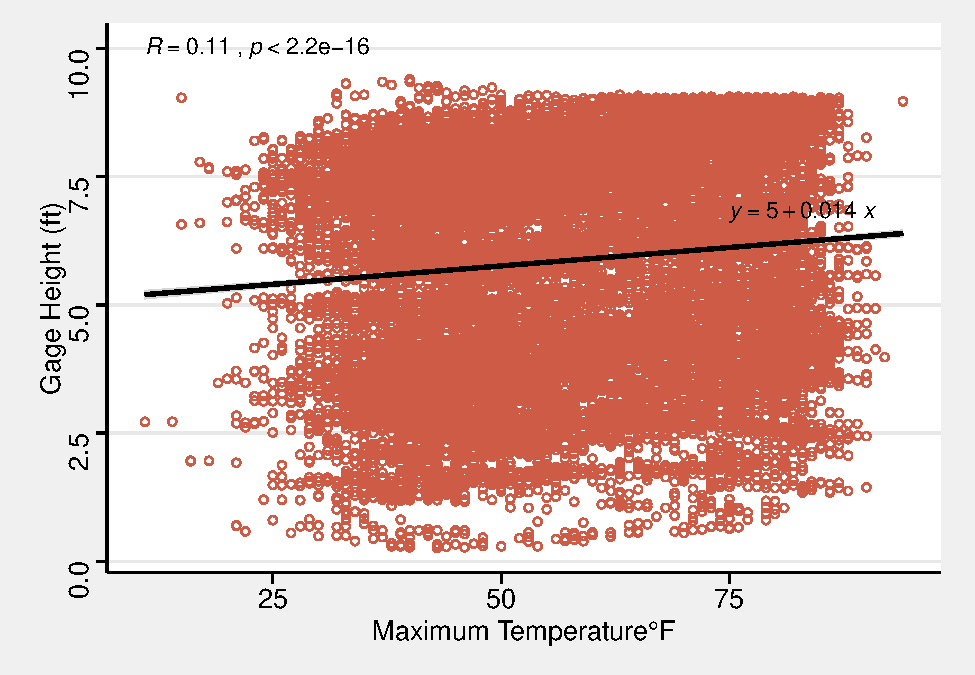
\includegraphics{Shintaku_ENV872_Project_files/figure-latex/unnamed-chunk-14-1.pdf}
\caption{Maximum temperature by gage height with trend line in black}
\end{figure}

\hypertarget{multiple-linear-regression}{%
\subsubsection{Multiple Linear
Regression}\label{multiple-linear-regression}}

\textbf{Multiple Linear Regression} is with a continuous response and
two or more continuous explanatory variables. Multiple linear regression
models were run on various combinations of the five climate variables.
However, with choosing variables yourself, it is possible to
over-parameterize a linear model so an Akaike's Information Criterion
(AIC) step regression was performed to find which explanatory variables
will predict the best gage height. Potential explanatory variables from
the dataset include precipitation, snowfall, snow depth, minimum
temperature, and maximum temperature.

\hypertarget{precipitation-snow-fall-and-minimum-temperature-as-significant-predictors}{%
\paragraph{Precipitation, Snow Fall, and Minimum Temperature as
Significant
Predictors}\label{precipitation-snow-fall-and-minimum-temperature-as-significant-predictors}}

A multiple linear regression was run on the variables precipiation,
minimum temperature, and snowfall indicating that all of the predictor
variables are significantly related to gage height (Multiple Linear
Regression, df = 22730, p-value = 2.2e-16, R2 = 0.026). For every 1 inch
increase in precipiation, there is a -0.14 ft decrease in gage height,
holding all other variables fixed. For every 1 degree F increase in
minimum temperature, there is a 0.033 ft increase in gage height,
holding all other variables fixed. Lastly, for every 1 inch increase in
snowfall, there is a 0.036 ft increase in gage height, holding all other
variables fixed. The adjusted R2 is 0.026 meaning that 2.6\% of the
variance in the measure of gage height can be predicted by
precipitation, minimum temperature, and snowfall.

\[GageHeight = 4.833 - 0.14*precipitation + 0.033*Tmin + 0.036*Snow   \]

\hypertarget{akaikes-information-criterion-step-regression}{%
\paragraph{Akaike's Information Criterion Step
Regression}\label{akaikes-information-criterion-step-regression}}

Akaike's Information Criterion (AIC) step regression was performed to
find which explanatory variables will predict the best gage height, and
the chosen model with the lowest AIC (34161) resulted in precipitation,
snow depth, maximum temperature, and minimum temperature being all
highly significant predictors of gage height (AIC, mutiple linear
regression, df = 22729, p-value = 2.2e-16, R2 = 0.038). For every 1 inch
increase in precipiation, there is a -0.31 ft decrease in gage height,
holding all other variables fixed. For every 1 inch increase in snow
depth, there is a 0.015 ft increase in gage height, holding all other
variables fixed. For every 1 degree F increase in minimum temperature,
there is a 0.067 ft increase in gage height, holding all other variables
fixed. Lastly, for every 1 degree F increase in maximum temperature,
there is a 0.021 ft decrease in gage height, holding all other variables
fixed. The adjusted R2 is 0.038 meaning that 3.8\% of the variance in
the measure of gage height can be predicted by precipitation, minimum
temperature, maximum temperature, and snow depth.

\[GageHeight = 4.86 - 0.31*precipitation + 0.015*snowdepth - 0.021*Tmax + 0.067*Tmin   \]

\newpage

\hypertarget{summary-and-conclusions}{%
\section{Summary and Conclusions}\label{summary-and-conclusions}}

Overall, this analysis led to a lot of valuable findings in how Lake
Tahoe's water level is changing over the years and what atmospheric
predictors play a key role in determining the water level. Using a time
series analysis, it was determined that there is a significant
decreasing trend over the time period of 1957-2019. Pettitt's change
detection test found four change points. Change point 1, 2, and 4 can be
traced back to specific drought events in California that may explain
why the lake level is drastically changing at those points. Droughts are
prolonged periods of low rainfall leading to shortages in water. With
precipitation and snowfall being the main contributors to lake level,
drought years would undoubtfully have adverse affects on lake level.
Climate change is intensifying droughts in California, which would then
impact atomspheric conditions and level of lake water.

After running through simple linear regression and multiple linear
regression methods, the highly significant climate predictors of lake
level are precipitation, snow depth, maximum daily temperature, and
minimum daily temperature. These results are taken from Akaike's
Information Criterion that returns the model with the lowest AIC and
best explanatory variables. These variables come at no surprise as
precipitation falls directly into the lake, and snow depth corresponds
to snow melt that flows into the lake. Daily min and max temperatures
also relate to weather events that cause precipitation and snow. It is
important to understand these drivers of lake level to protect Tahoe's
surrounding ecosystem in the face of climate change as well as monitor
the legal water level limit.

This preliminary study provides a baseline for further research in
understanding how atomspheric factors play a role in Lake Tahoe's
overall ecosystem. Further analysis could explore variables such as,
water quality, water clarity, nutrients levels, water temperature, and
algal biomass. There are a lot more factors to consider than just
climate when quantifying a trend in lake level.


\end{document}
